%% Exemplo de utilizacao do estilo de formatacao normas-utf-tex (http://normas-utf-tex.sourceforge.net)
%% Autores: (200?-2011) Hugo Vieira Neto (hvieir@utfpr.edu.br)
%%          (200?-2011) Diogo Rosa Kuiaski (diogo.kuiaski@gmail.com)
%%          (2011-2012) Marcos Talau <talau@users.sourceforge.net>
%% Colaborador:
%%          (2011) César M. Vargas Benitez <cesarvargasb@gmail.com>

\documentclass[openright]{normas-utf-tex} %openright = o capitulo comeca sempre em paginas impares
%\documentclass[oneside]{normas-utf-tex} %oneside = para dissertacoes com numero de paginas menor que 100 (apenas frente da folha) 

% force A4 paper format
\special{papersize=210mm,297mm}

\usepackage[alf,abnt-emphasize=bf,bibjustif,recuo=0cm, abnt-etal-cite=2, abnt-etal-list=99]{abntcite} %configuracao correta das referencias bibliograficas.

\usepackage[brazil]{babel} % pacote portugues brasileiro
\usepackage[utf8]{inputenc} % pacote para acentuacao direta
\usepackage{amsmath,amsfonts,amssymb} % pacote matematico
\usepackage{graphicx} % pacote grafico
\usepackage{times} % fonte times
\usepackage[final]{pdfpages} % adicao da ata
\usepackage{epigraph}
\usepackage{chngcntr}
%\usepackage{subfigure}
\usepackage{caption}
\usepackage{subcaption}

%Podem utilizar GEOMETRY{...} para realizar pequenos ajustes das margens. Onde, left=esquerda, right=direita, top=superior, bottom=inferior. P.ex.:
%\geometry{left=3.0cm,right=1.5cm,top=4cm,bottom=1cm} 

% ---------- Preambulo ----------
\instituicao{Universidade Tecnológica Federal do Paraná}
\programa{Programa de Pós-Graduação em Engenharia Elétrica e Informática Industrial}
%\area{}

\documento{Dissertação}
\nivel{Mestrado}
\titulacao{Mestre}

\titulo{{Título em português}} % titulo do trabalho em portugues
\title{\MakeUppercase{Title in English}} % titulo do trabalho em ingles

\autor{Daniel Alexandre Oleinik} % autor do trabalho
\cita{OLEINIK, Daniel Alexandre} % sobrenome (maiusculas), nome do autor do trabalho

\palavraschave{\emph{Smart Grid}, Chaveador óptico, Redes IP, Redes \emph{Mesh}, Otimização, Latência, Algoritmos Genéticos} % palavras-chave do trabalho
\keywords{\emph{Smart Grid, Optical Switch, IP networks, Mesh networks, Optimization, Latency, Genetic Algorithms}} % palavras-chave do trabalho em ingles

\comentario{Dissertação apresentada ao Programa de Pós-graduação em Engenharia Elétrica e Informática Industrial da Universidade Tecnológica Federal do Paraná como requisito parcial para obtenção do grau ``Mestre em Ciências'' - Área de Concentração: Informática Industrial}

\orientador{Mauro Sergio Pereira Fonseca} % nome do orientador do trabalho
%\orientador[Orientadora:]{Nome da Orientadora} % <- no caso de orientadora, usar esta sintaxe
%\coorientador{Nome do Co-orientador} % nome do co-orientador do trabalho, caso exista
%\coorientador[Co-orientadora:]{Nome da Co-orientadora} % <- no caso de co-orientadora, usar esta sintaxe
%\coorientador[Co-orientadores:]{Nome do Co-orientador} % no caso de 2 co-orientadores, usar esta sintaxe
%\coorientadorb{Nome do Co-orientador 2}	% este comando inclui o nome do 2o co-orientador

\local{Curitiba} % cidade
\data{\the\year} % ano automatico

% desativa hifenizacao mantendo o texto justificado.
% thanks to Emilio C. G. Wille
\tolerance=1
\emergencystretch=\maxdimen
\hyphenpenalty=10000
\hbadness=10000
\sloppy

%---------- Inicio do Documento ----------
\begin{document}

\capa % geracao automatica da capa
\folhaderosto % geracao automatica da folha de rosto

% Lembre-se de que a ficha catalografica eh impressa no verso da folha de rosto
% Ficha catalografica
\fichacatpum{T137}
\fichacatautor{Sobrenome, Nome}
\fichacatpgbib{\pageref{bibstart}-\pageref{bibend}}
\fichacatpalcha{1. Teoria do controle. 2. Redes de comutação. 3. TCP/IP (Protocolo de rede de computação), ...}
\fichacatpdois{CDD (22. ed.) 621.3}
\fichacatbib{Biblioteca Dois Vizinhos}
\fichacat

% insercao da ATA
%\includepdf{ata.pdf}

% dedicatoria
%\begin{dedicatoria}
%Texto da dedicatória.
%\end{dedicatoria}
%
%% agradecimentos (opcional)
%\begin{agradecimentos}
%Texto dos agradecimentos.
%\end{agradecimentos}

% epigrafe (opcional)
\begin{epigrafe}
\epigraph{\emph{``Muito melhor é o homem paciente que o guerreiro, mais vale controlar as emoções e os ímpetos do que conquistar toda uma cidade!''}}{Provérbios 16:32}
\end{epigrafe}

%resumo
\begin{resumo}
O crescente consumo de energia proveniente de fontes não renováveis e finitas vem incentivando o avanço no desenvolvimento e utilização de novas opções de geração de energia. Estas opções, quando incorporadas ao sistema atual de geração e distribuição de energia elétrica, devem demandar novas exigências do sistema de comunicação utilizado entre os equipamentos da rede, motivando o desenvolvimento do \emph{Smart Grid} (SG). O presente documento propõe um método para melhoria e otimização de uma rede, ou grid, de acesso construída em fibra óptica com topologia \emph{mesh}, através de alterações das conexões físicas da rede em conjunto com uma gerência reativa inteligente.
\end{resumo}

%abstract
\begin{abstract}
The increasing consumption of energy from nonrenewable and finite sources is encouraging the advance of development and use
of new energy generation options. These options, when incorporated into the current electricity generation and distribution system,
should demand new requirements from the communication system used to provide the communication link between the network
equipment used, motivating the development of Smart grid. This document proposes a method to improve and optimize the network
or grid access, built with optic fiber and mesh topology through the handling of the physical connections in the network together with
a smart reactive management.
\end{abstract}

% listas (opcionais, mas recomenda-se a partir de 5 elementos)
\listadefiguras % geracao automatica da lista de figuras
\listadetabelas % geracao automatica da lista de tabelas
\listadequadros % adivinhe :)
\listadesiglas % geracao automatica da lista de siglas
\listadesimbolos % geracao automatica da lista de simbolos

% sumario
\sumario % geracao automatica do sumario


%---------- Inicio do Texto ----------
% recomenda-se a escrita de cada capitulo em um arquivo texto separado (exemplo: intro.tex, fund.tex, exper.tex, concl.tex, etc.) e a posterior inclusao dos mesmos no mestre do documento utilizando o comando \input{}, da seguinte forma:
%\input{intro.tex}
%\input{fund.tex}
%\input{exper.tex}
%\input{concl.tex}


\setcounter{page}{12}

%---------- Primeiro Capitulo ----------
\input{introducao.tex}

\counterwithout{figure}{chapter}% Continuous numbering of figures
%---------- Segundo Capitulo ----------
\chapter{Fundamentação Teórica}
Este capítulo apresenta conceitos utilizados no desenvolvimento do trabalho, e portanto necessários para o correto entendimento do mesmo.

\section{Redes de Computadores}
A história dos computadores de grande escala começa em fevereiro de 1946 através da invenção do primeiro ``computador integrador numérico eletrônico'' \sigla{ENIAC}{\emph{Electronic Numerical Integrator and Computer}} \cite{Book-Jean2013}. Ele começou a ser desenvolvido anos antes, durante a Segunda Guerra Mundial, com a principal tarefa de auxiliar nos cálculos necessários para o fronte de batalha.

Em meados dos anos 50, com a popularização dos transistores, foi possível realizar uma imensa miniaturização dos circuitos eletrônicos possibilitando a criação de máquinas com altíssimo poder de processamento em um tamanho extremamente reduzido. Além disso, essas máquinas tornaram-se cada vez mais robustas e baratas, fazendo com que a posse e utilização de computadores pudesse ser disseminada alcançando os patamares atuais.

Neste sentido foi natural a necessidade da troca de informações/dados entre os diversos computadores existentes, o que claramente não representa maiores problemas caso os equipamentos em questão estejam fisicamente perto uns dos outros. Em contrapartida, é fácil imaginar a dificuldade de realização desta tarefa no caso em que estes equipamentos estão fisicamente distantes. Este é o cerne do problema que motivou a criação das redes de computadores.

Segundo \cite{Book-Kurose2013} uma rede de computadores nada mais é do que uma infraestrutura de comunicação que fornece serviços à aplicações distribuídas através de \emph{links} de comunicação contendo ``chaveadores de pacotes''. Sendo que uma rede pode ser essencialmente definida por seu tamanho, topologia e tecnologia de transmissão utilizada \cite{Book-Tanenbaum2003}. 
%Essas características, apesar de presentes em qualquer rede, são especialmente aplicáveis a redes locais (comumente chamadas de \sigla{LAN}{\emph{Local Area Network}}). 

\subsection{Tamanho}
Segundo \cite{Book-Tanenbaum2003} uma \sigla{LAN}{\emph{Local Area Network}} ou Rede Local possui tamanho restrito, e por isso seu desempenho é previsível. Ou seja, os piores tempos de transmissão de pacotes são conhecidos. 

Este tipo de rede pode possuir diversas topologias diferentes e pode ser encontrada nas mais diversas aplicações, desde residenciais, até industriais ou de automação. Uma das suas principais vantagens é a previsibilidade em termos de latência, visto que além de limitada e completamente conhecida ela normalmente não sofre alterações frequentes.

Uma Rede Metropolitana ou \sigla{MAN}{Metropolitan Area Network}, por sua vez, abrange uma cidade. Redes como esta foram inicialmente instaladas para sinais de TV a cabo. Atualmente elas são também utilizadas por provedores de internet \cite{Book-Tanenbaum2003}.

Uma Rede Geograficamente Distribuída ou \sigla{WAN}{Wide Area Network} abrange uma grande região como um país ou um continente e é responsável pelo roteamento dos pacotes entre as redes origem e destino. A forma e caminho utilizados para enviar as informações neste processo depende do algoritmo de roteamento utilizado. \cite{Book-Tanenbaum2003}

\subsection{Topologia}
Existem diversas formas de realizar a interconexão entre \emph{hosts} (dispositivos finais ou \emph{endpoints}). A topologia da rede depende de como esta interconexão é realizada. De maneira geral, podem-se destacar como mais comuns as topologias em barramento, anel, estrela, árvore e \emph{mesh}.

Uma topologia em barramento compartilha um mesmo meio para diversos \emph{hosts}. Todas as vezes que um deles deseja enviar alguma informação todos os equipamentos a recebem mas apenas o destinatário final à utiliza. Visto que o meio de comunicação é compartilhado é necessário existir alguma política de controle de acesso ao meio, prevenindo que mais de um \emph{endpoint} envie dados ao mesmo tempo, o que poderia gerar uma ``colisão'' embaralhando os dados de ambas as fontes. Este controle fica sob responsabilidade do protocolo de comunicação utilizado. A Figura \ref{fig_topologia_multiplo_barramento} representa uma rede conectada em barramento, percebe-se que o barramento central é compartilhado entre os diversos dispositivos conectados.

%\begin{figure}[!htb]
	%\centering
	%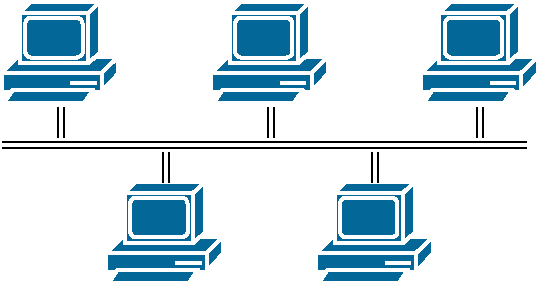
\includegraphics[width=0.2\textwidth]{./figuras/Topologia-Barramento.pdf} % <- formatos PNG, JPG e PDF
	%\caption[Exemplo de topologia em barramento]{Exemplo de topologia conectada em barramento. Percebe-se que o barramento central é compartilhado entre os diversos dispositivos conectados.}
	%\label{fig_topologia_barramento}
%\end{figure}

Na topologia em anel os \emph{hosts} são conectados através de um \emph{link} fechado, criando um anel. Cada estação é responsável por receber os dados em uma porta e encaminhá-los à outra até que este alcance seu destino. Neste tipo de topologia as colisões de dados são menos frequentes, visto que cada ``perna'' do \emph{link} é estabelecida entre apenas dois \emph{hosts}, em contrapartida o protocolo utilizado precisa tratar a dinâmica de recepção e retransmissão de dados entre todos os \emph{links}. Este tipo de rede fornece redundância já que as mensagens trocadas podem ser enviadas por mais de um caminho. A Figura \ref{fig_topologia_multiplo_barramento_anel} representa uma rede em anel, pode-se perceber que neste caso todos os equipamentos fazem parte da rede e precisam repetir os dados recebidos para os demais.

%\begin{figure}[!htb]
	%\centering
	%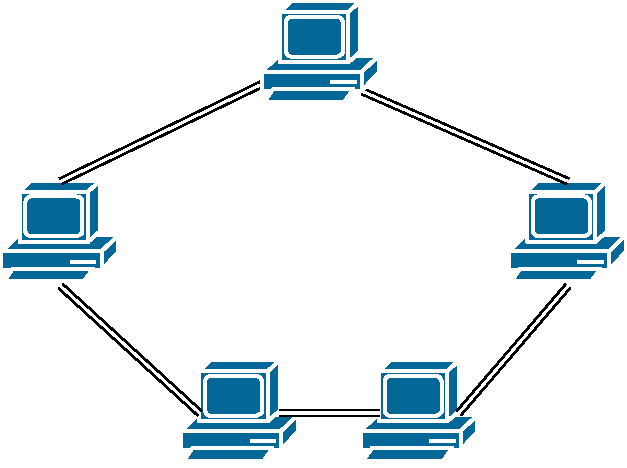
\includegraphics[width=0.2\textwidth]{./figuras/Topologia-Anel.pdf} % <- formatos PNG, JPG e PDF
	%\caption[Exemplo de topologia em anel]{Exemplo de topologia conectada em anel. Percebe-se que todos os equipamentos fazem parte da rede e precisam repetir os dados recebidos para os demais.}
	%\label{fig_topologia_anel}
%\end{figure}

A topologia estrela é muito utilizada em redes sem fio, visto que de maneira geral, todos os \emph{hosts} estão conectados a um ponto de acesso ou \sigla{AP}{Access Point}. Esse tipo de rede também pode ser facilmente encontrada em um meio cabeado, como no caso da utilização dos roteadores/switches residenciais, onde todos os \emph{hosts} são conectados a um mesmo equipamento responsável pela criação de uma LAN e interconexão com uma WAN. A Figura \ref{fig_topologia_multiplo_estrela} representa uma rede de topologia estrela, neste tipo de topologia todos os equipamentos estão ligados a um nó central, neste caso um \emph{switch}.

%\begin{figure}[!htb]
	%\centering
	%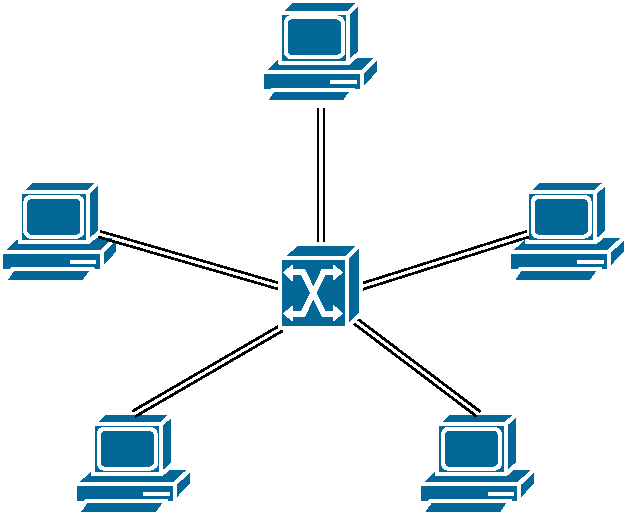
\includegraphics[width=0.2\textwidth]{./figuras/Topologia-Estrela.pdf} % <- formatos PNG, JPG e PDF
	%\caption[Exemplo de topologia em estrela]{Exemplo de topologia conectada em estrela. Percebe-se que todos os equipamentos estão ligados a um nó central, neste caso um \emph{switch}.}
	%\label{fig_topologia_estrela}
%\end{figure}

A topologia em árvore, talvez a mais recorrente em redes de computadores, é assim chamada pois pode ser reconhecida pelo seu aspecto onde o nó central representa a base da árvore e os diversos \emph{hosts} representam suas folhas (normalmente representada como uma árvore invertida). Basicamente trata-se de uma estrutura hierárquica de conexão entre várias redes e/ou sub-redes. A Figura \ref{fig_topologia_multiplo_arvore} ilustra esse tipo de topologia. Percebe-se que a topologia assemelha-se à interconexão de várias sub-redes através de equipamentos dedicados.

%\begin{figure}[!htb]
	%\centering
	%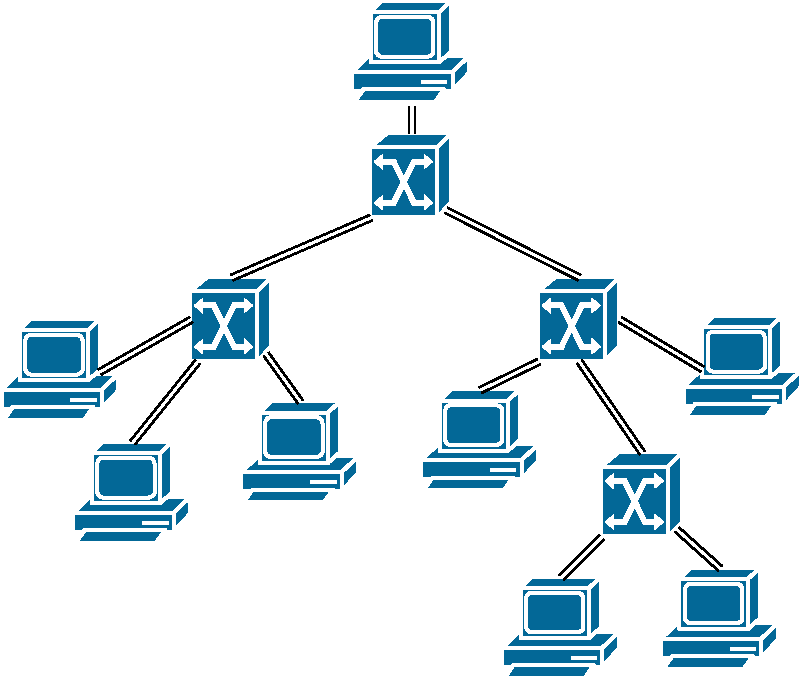
\includegraphics[width=0.2\textwidth]{./figuras/Topologia-Arvore.pdf} % <- formatos PNG, JPG e PDF
	%\caption[Exemplo de topologia em árvore]{Exemplo de topologia conectada em árvore. Percebe-se que a topologia assemelha-se à interconexão de várias sub-redes através de equipamentos dedicados.}
	%\label{fig_topologia_arvore}
%\end{figure}

A topologia em malha ou \emph{mesh} por sua vez, é caracterizada pela criação de uma rede grandemente (podendo chegar a ser plenamente) interconectada, formando diversos caminhos redundantes para a interligação entre a origem e o destino das mensagens. Fato que confere a este tipo de rede um elevado grau de disponibilidade, visto que mesmo em caso de falha de equipamentos ou da infraestrutura a comunicação não é necessariamente comprometida. A Figura \ref{fig_topologia_multiplo_mesh} ilustra uma rede \emph{mesh}. É possível notar que existem diversas rotas redundantes devido aos vários links estabelecidos entre os equipamentos da rede.

%\begin{figure}[!htb]
	%\centering
	%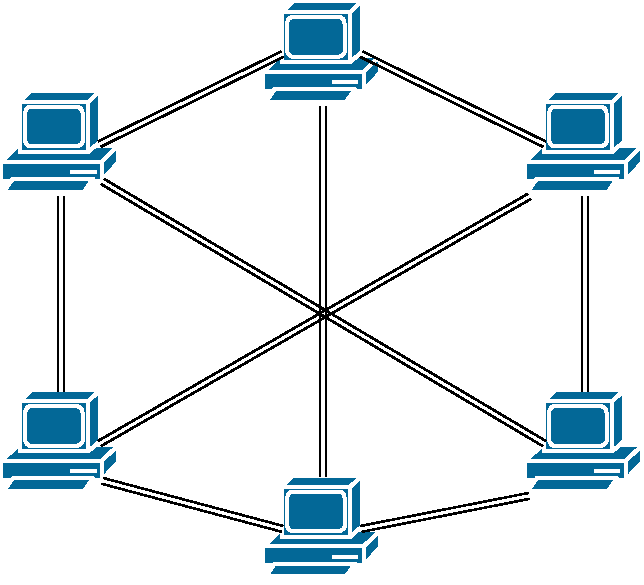
\includegraphics[width=0.2\textwidth]{./figuras/Topologia-Mesh.pdf} % <- formatos PNG, JPG e PDF
	%\caption[Exemplo de topologia em \emph{mesh}]{Exemplo de topologia conectada em \emph{mesh}. Percebe-se existem diversas rotas redundantes devido aos vários links estabelecidos entre os equipamentos da rede.}
	%\label{fig_topologia_mesh}
%\end{figure}

\begin{figure}[t!]
	\centering
	\begin{subfigure}[t]{0.4\textwidth}
		\centering
		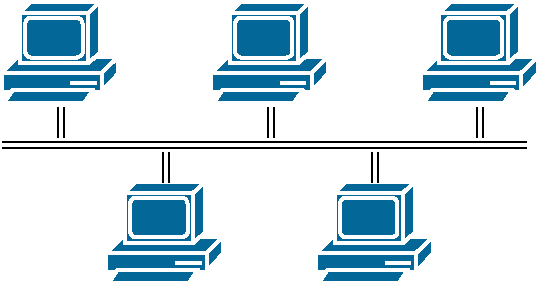
\includegraphics[width=4cm]{./figuras/Topologia-Barramento.pdf} % <- formatos PNG, JPG e PDF
		\caption{Topologia em barramento.}
		\label{fig_topologia_multiplo_barramento}
	\end{subfigure}%
	~
	\begin{subfigure}[t]{0.4\textwidth}
		\centering
		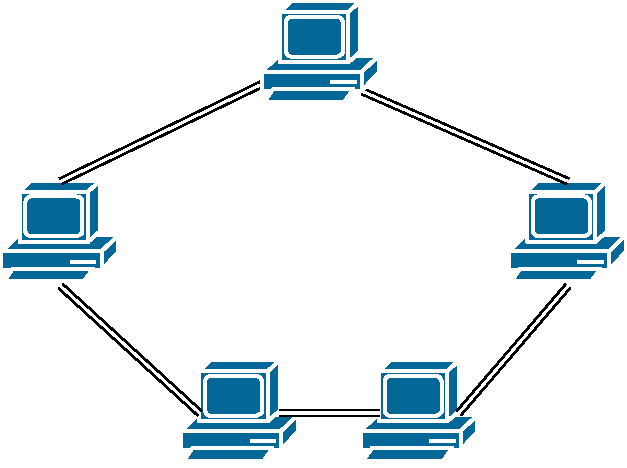
\includegraphics[width=4cm]{./figuras/Topologia-Anel.pdf} % <- formatos PNG, JPG e PDF
	\caption{Topologia em anel.}
	\label{fig_topologia_multiplo_barramento_anel}
	\end{subfigure}
	~
	\begin{subfigure}[t]{0.4\textwidth}
		\centering
		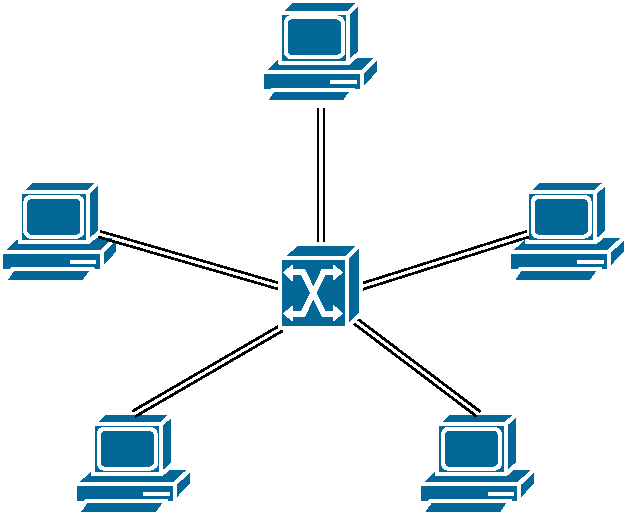
\includegraphics[width=4cm]{./figuras/Topologia-Estrela.pdf} % <- formatos PNG, JPG e PDF
	\caption{Topologia em estrela.}
	\label{fig_topologia_multiplo_estrela}
	\end{subfigure}
	~
	\begin{subfigure}[t]{0.4\textwidth}
		\centering
		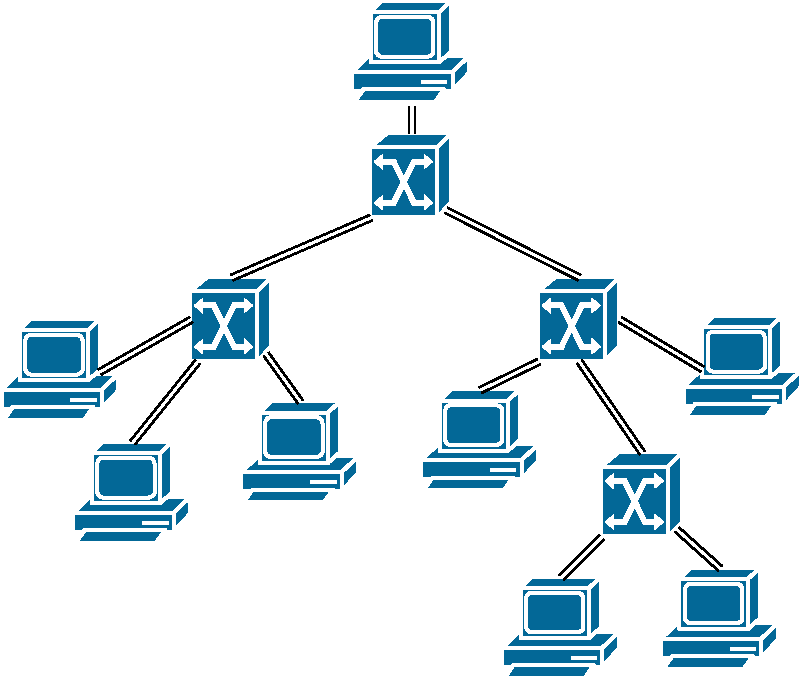
\includegraphics[width=4cm]{./figuras/Topologia-Arvore.pdf} % <- formatos PNG, JPG e PDF
	\caption{Topologia em árvore.}
	\label{fig_topologia_multiplo_arvore}
	\end{subfigure}
	~
	\begin{subfigure}[t]{0.4\textwidth}
		\centering
		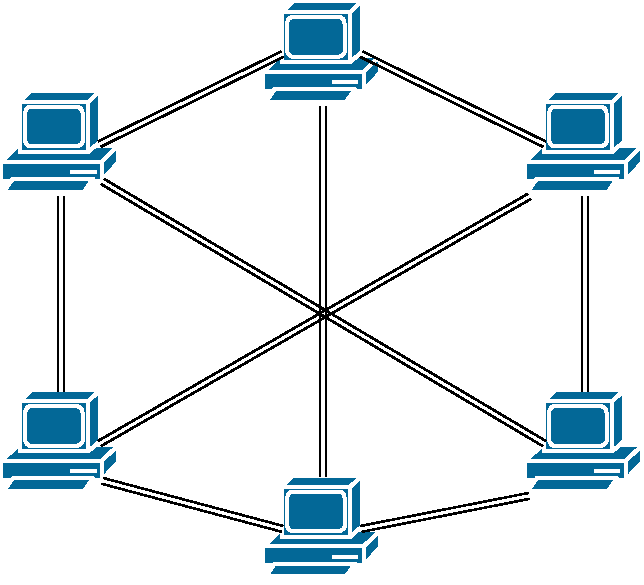
\includegraphics[width=4cm]{./figuras/Topologia-Mesh.pdf} % <- formatos PNG, JPG e PDF
	\caption{Topologia em \emph{mesh}.}
	\label{fig_topologia_multiplo_mesh}
	\end{subfigure}
	\caption{Tipos básicos de topologia}
	\label{fig_topologia_multiplo}
\end{figure}

\subsection{Tecnologia de Transmissão}
A tecnologia de transmissão está diretamente ligada ao meio físico utilizado, que não precisa ser necessariamente construído em cabos metálicos. Podem ser utilizados fibras ópticas, enlaces de micro-ondas, ondas infravermelhas, satélites de comunicação, entre outros \cite{Book-Tanenbaum2003}. 

Além disso, as redes de computadores podem, e comumente são, criadas através da interconexão de redes híbridas, ou seja, diferentes sub-redes criadas com tecnologias de transmissão distintas. Essas redes por sua vez têm diferentes taxas de transmissão e valores típicos de latência e demais parâmetros aos quais todos os pacotes que as atravessarem estarão submetidos \cite{Book-Kurose2013}. Logo, quando é necessário realizar uma comunicação entre \emph{hosts} em redes que utilizam tecnologias de transmissão diferentes é necessária a existência de algum tipo de mecanismo para regulação da velocidade de transferência de informação assim como políticas de garantia de entrega dos dados. Estes mecanismos são algumas das responsabilidades básicas dos protocolos de roteamento como o TCP/IP.

\subsection{Comutadores Ópticos}
A comunicação em redes ópticas é feita através da modulação de sinais luminosos, cada um desses sinais possui uma frequência diferente (usualmente também chamada de cor do sinal) o que implica em diferentes comprimentos de onda (\simbolo{$\lambda$}{comprimento de onda}). Redes complexas e com grande número de $\lambda$s  como as redes ópticas atuais, possuem em seus nós centrais equipamentos conhecidos como comutadores ópticos, também chamados de \sigla{OXC}{Optical Cross Connect}. OXCs podem realizar roteamento interno de sinais de maneira puramente óptica, puramente elétrica ou até mesmo híbrida\cite{Book-Ramaswami2010}. Existem basicamente três diferentes classificações de equipamentos OXC, os opacos, os transparentes e os translúcidos.
%Usar Optical Networks pagina 488
OXC opacos são assim chamados por impedirem a passagem direta da luz, ou seja, o roteamento que esse tipo de equipamento oferece é realizado no domínio elétrico. Para isso todos os sinais que entram no equipamento são convertido em sinais elétricos e enviados a um \emph{switch} ou processador eletrônico que fará o devido roteamento, para que então esses sinais sejam novamente convertidos em sinais ópticos através da utilização de \emph{transceivers} e lasers. Este tipo de equipamento é amplamente empregado em redes ópticas atuais e são muitas vezes conhecidos como \sigla{OEO}{Optical-Electrical-Optical} ou Óptico-Elétrico-Óptico em tradução livre.

Equipamentos OXC opacos possuem o inconveniente de que a circuitaria eletrônica utilizada acaba por limitar a banda do sinal. Existem diversas razões para esta limitação sendo as principais delas as conversões de meio necessárias e o poder de processamento do próprio equipamento. Apesar disso, a grande vantagem deste tipo de equipamento reside no custo benefício, já que ele possibilita a regeneração do sinal óptico a cada nó da rede, visto que o sinal precisa ser recriado, e o controle e obtenção de métricas relativas à comunicação transportada por ele.  

OXC transparentes por sua vez, são assim chamados por não interromperem o sinal de luz que os transpassa. Esse tipo de equipamento tem a capacidade de realizar a separação dos comprimentos de onda de luz e seu devido encaminhamento ou roteamento para a interface desejada. 

Em linhas gerais, a luz que chega ao equipamento (composta por diferentes $\lambda$s) é demultiplexada de acordo com a sua cor ou $\lambda$, direcionada para a saída desejada e unida aos demais sinais luminosos da respectiva saída através de um multiplexador, para então serem enviados através de uma fibra óptica. 

Percebe-se que este tipo de equipamento faz a divisão e roteamento de luz em grande parte de maneira passiva, alterando o menos possível os sinais que por ele transitam (normalmente o efeito mais significativo sobre o sinal está relacionado à potência e separação de $\lambda$s do mesmo), logo o sinal não é demodulado/interpretado impedindo a obtenção de métricas de qualidade ou controle sobre a comunicação. Além disso, estes equipamentos costumam ter sua performance grandemente atrelada a dispositivos sensíveis, como filtros internos, o que acarreta em um custo final elevado. A Figura \ref{fig_oxc_optico} contém o diagrama básico de um OXC transparente. Razões estas que impedem sua ampla utilização em redes ópticas de grande porte.

\begin{figure}[!htb]
	\centering
	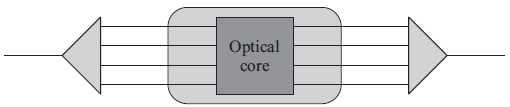
\includegraphics[width=0.5\textwidth]{./figuras/OXC-Optico.png} % <- formatos PNG, JPG e PDF
	\caption[Exemplo básico de OXC óptico]{Exemplo básico de um equipamento OXC transparente. Percebe-se que o sinal de entrada é apenas repassado à respectiva saída sem nenhuma outra intervenção.}
	\fonte{\cite{Book-Ramaswami2010}}
	\label{fig_oxc_optico}
\end{figure}

Por fim, um OXC translúcido traduz-se em um equipamento que representa um compromisso entre os dois tipos anteriores. Ou seja, um equipamento de roteamento em redes ópticas que tem a capacidade de processamento de pacotes e de chaveamento de luz. Este tipo de equipamento, apesar de não ser comumente encontrado, é o foco do presente trabalho.

A proposta que será detalhadamente descrita no Capítulo \ref{capitulo_proposta} pode ser usada para transformar um equipamento óptico seja qual for em um equipamento similar a um OXC translúcido através da utilização de chaveadores ópticos ou \emph{switches} ópticos.

Chaveadores ópticos são componentes capazes de desviar um feixe luminoso através da utilização de um prisma refletor. A Figura \ref{fig_chaveador_optico} mostra o diagrama interno simplificado de um chaveador óptico, percebe-se que seu funcionamento é análogo ao de um relé elétrico.

\begin{figure}[!htb]
	\centering
	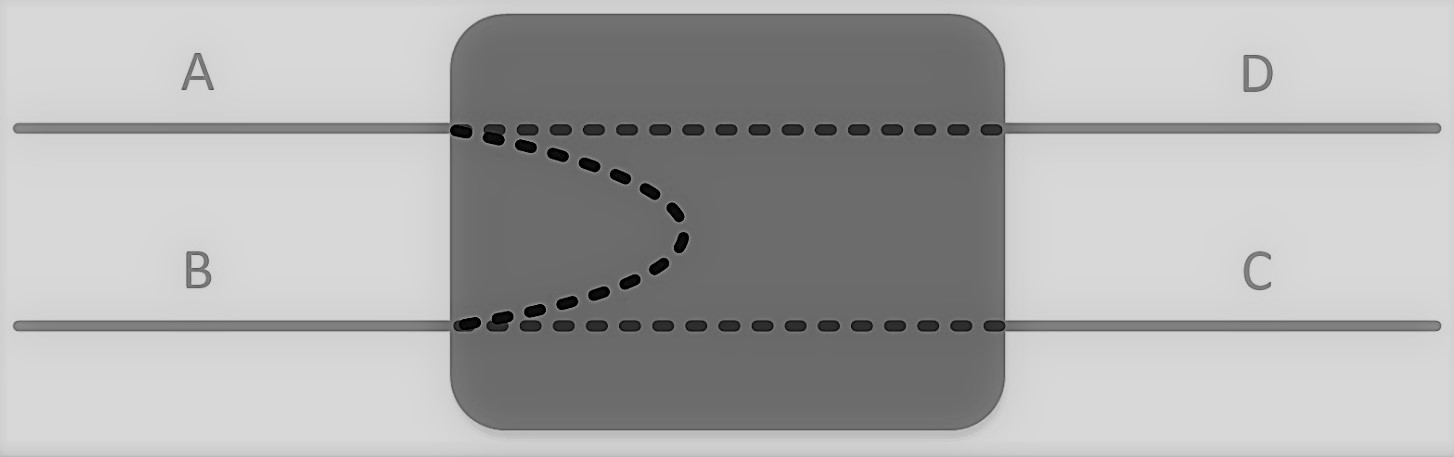
\includegraphics[width=0.5\textwidth]{./figuras/Switch_optico.jpg} % <- formatos PNG, JPG e PDF
	\caption[Exemplo básico chaveador óptico]{Diagrama interno simplificado de um chaveador óptico. Em um estado este componente transmite bidirecionalmente a luz da interface A para D e B para C, quando acionado ele transmite bidirecionalmente a luz da interface A para B.}
	\fonte{Adaptado de \cite{Accelink2014}}
	\label{fig_chaveador_optico}
\end{figure}

A utilização de um chaveador óptico em conjunto com um equipamento OEO pode conferir-lhe a capacidade de desviar sinais ópticos caso necessário, surgindo assim um equipamento de roteamento que pode ser classificado como sendo um OXC 
\section{Protocolos de Roteamento}
\label{cap_protocolos_de_roteamento}
Este capítulo destina-se à discussão de alguns dos protocolos de roteamento recorrentemente utilizados no cenário descrito.

\subsection{Definição de Protocolo}
Assim como no mecanismo formal de troca de informações entre humanos um protocolo de comunicação é o que estabelece as regras básicas para troca de dados entre máquinas. Segundo \cite{Book-Kurose2013} um procolo de comunicação define o formato e a ordem das mensagens trocadas entre duas ou mais entidades, assim como as ações necessárias para que esses dados sejam corretamente recebidos/enviados. A Figura \ref{fig_explicacao_protocolo} exemplifica este paralelo.

\begin{figure}[!htb]
	\centering
	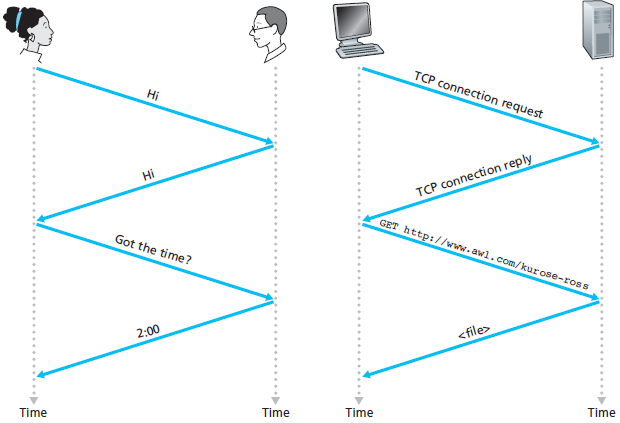
\includegraphics[width=0.5\textwidth]{./figuras/Explicacao-Protocolo.png} % <- formatos PNG, JPG e PDF
	\caption[Exemplo de Protocolo de Comunicação]{Exemplo de Protocolo de Comunicação, o paralelo entre o mecanismo de comuniacação entre humanos e um protocolo de comunicação entre máquinas exemplifica a definição de ``protocolo''.}
	\fonte{\cite{Book-Kurose2013}}
	\label{fig_explicacao_protocolo}
\end{figure}

Um protocolo de comunicação pode ser implementado em software, hardware ou em uma combinação de ambos. De maneira geral, eles são convenientemente separados em camadas ou \emph{layers}, que por sua vez oferecem ``serviços'' aos \emph{layers} superiores \cite{Book-Kurose2013}. Esses \emph{layers} são normalmente baseados em um modelo conhecido como Modelo de Referencia \sigla{OSI}{\emph{Open Systems Interconnection}} convenientemente representado na Figura \ref{fig_modelo_OSI}. Essa modularidade é extremamente útil visto que fornece um nível de abstração interessante aos protocolos, possibilitando por exemplo que o mesmo protocolo possa ser utilizado independentemente do meio físico em questão.

\begin{figure}[!htb]
	\centering
	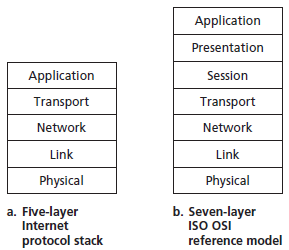
\includegraphics[width=0.4\textwidth]{./figuras/Modelo-OSI.png} % <- formatos PNG, JPG e PDF
	\caption[Modelo OSI]{Comparação entre o Modelo de Referência OSI e a pilha de protocolos de Internet.}
	\fonte{\cite{Book-Kurose2013}}
	\label{fig_modelo_OSI}
\end{figure}

\subsection{Descrever protocolos comuns???}

%\chapter{Desenvolvimento}
%\label{chap:desenv}
%
%A seguir ilustra-se a forma de incluir figuras, tabelas, equa\c{c}\~oes, siglas e s\'imbolos no documento, obtendo indexa\c{c}\~ao autom\'atica em suas respectivas listas. A numera\c{c}\~ao sequencial de figuras, tabelas e equa\c{c}\~oes ocorre de modo autom\'atico. Refer\^encias cruzadas s\~ao obtidas atrav\'es dos comandos {\ttfamily \textbackslash label\{\}} e {\ttfamily \textbackslash ref\{\}}. Por exemplo, n\~ao \'e necess\'ario saber que o n\'umero deste cap\'itulo \'e~\ref{chap:desenv} para colocar o seu n\'umero no texto. Isto facilita muito a inser\c{c}\~ao, remo\c{c}\~ao ou reloca\c{c}\~ao de elementos numerados no texto (fato corriqueiro na escrita e corre\c{c}\~ao de um documento acad\^emico) sem a necessidade de renumer\'a-los todos.
%
%\section{Figuras}
%
%Na figura~\ref{fig:dummy} \'e apresentado um exemplo de gr\'afico flutuante. Esta figura aparece automaticamente na lista de figuras. Para uso avan\c{c}ado de gr\'aficos no \LaTeX, recomenda-se a consulta de literatura especializada~\cite{Goossens2007}.
%
%
%\begin{figure}[!htb]
	%\centering
	%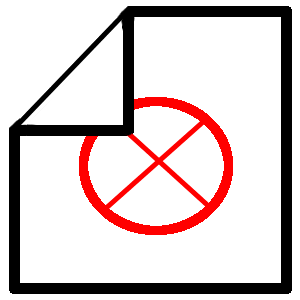
\includegraphics[width=0.2\textwidth]{./figuras/dummy.png} % <- formatos PNG, JPG e PDF
	%\caption[Exemplo de uma figura]{Exemplo de uma figura onde aparece uma imagem sem nenhum significado especial.}
	%\fonte{\cite{abnTeX2009}}
	%\label{fig:dummy}
%\end{figure}
%
%
%\section{Tabelas}
%
%Tamb\'em \'e apresentado o exemplo da tabela~\ref{tab:correlacao}, que aparece automaticamente na lista de tabelas. Informa\c{c}\~oes sobre a constru\c{c}\~ao de tabelas no \LaTeX\ podem ser encontradas na literatura especializada~\cite{Lamport1986,Buerger1989,Kopka2003,Mittelbach2004}.
%
%\begin{table}[!htb]
	%\centering
	%\caption[Exemplo de uma tabela]{Exemplo de uma tabela mostrando a correla\c{c}\~ao entre x e y.}
	%\label{tab:correlacao}
	%\begin{tabular}{cc}
		%\hline 
		%x & y \\
		%\hline
		%1 & 2 \\
		%3 & 4 \\
		%5 & 6 \\
		%7 & 8 \\
		%\hline 
	%\end{tabular}
	%\fonte{Autoria pr\'opria.}
%\end{table}
%
%\section{Equa\c{c}\~oes}
%
%A transformada de Laplace \'e dada na equa\c{c}\~ao~(\ref{eq:laplace}), enquanto a equa\c{c}\~ao~(\ref{eq:dft}) apresenta a formula\c{c}\~ao da transformada discreta de Fourier bidimensional\footnote{Deve-se reparar na formata\c{c}\~ao esteticamente perfeita destas equa\c{c}\~oes!}.
%
%\begin{equation}
%X(s) = \int\limits_{t = -\infty}^{\infty} x(t) \, \text{e}^{-st} \, dt
%\label{eq:laplace}
%\end{equation}
%
%\begin{equation}
%F(u, v) = \sum_{m = 0}^{M - 1} \sum_{n = 0}^{N - 1} f(m, n) \exp \left[ -j 2 \pi \left( \frac{u m}{M} + \frac{v n}{N} \right) \right]
%\label{eq:dft}
%\end{equation}
%
%\section{Siglas e s\'imbolos}
%
%O pacote \textsc{abn}\TeX\ permite ainda a defini\c{c}\~ao de siglas e s\'imbolos com indexa\c{c}\~ao autom\'atica atrav\'es dos comandos {\ttfamily \textbackslash sigla\{\}\{\}} e {\ttfamily \textbackslash simbolo\{\}\{\}}. Por exemplo, o significado das siglas\sigla{CPGEI}{Programa de P\'os-gradua\c{c}\~ao em Engenharia El\'etrica e Inform\'atica Industrial},\sigla{DAELN}{Departamento Acad\^emico de Eletr\^onica} e\sigla{UTFPR}{Universidade Tecnol\'ogica Federal do Paran\'a} aparecem automaticamente na lista de siglas, bem como o significado dos s\'imbolos\simbolo{$\lambda$}{comprimento de onda},\simbolo{$v$}{velocidade} e\simbolo{$f$}{frequ\^encia} aparecem automaticamente na lista de s\'imbolos. Mais detalhes sobre o uso destes e outros comandos do \textsc{abn}\TeX\ s\~ao encontrados na sua documenta\c{c}\~ao espec\'ifica~\cite{abnTeX2009}.


%---------- Terceiro Capitulo ----------
\chapter{Conclus\~ao}

%Espera-se que o uso do estilo de formata\c{c}\~ao \LaTeX\ adequado \`as Normas para Elabora\c{c}\~ao de Trabalhos Acad\^emicos da UTFPR ({\ttfamily normas-utf-tex.cls}) facilite a escrita de documentos no \^ambito desta institui\c{c}\~ao e aumente a produtividade de seus autores. Para usu\'arios iniciantes em \LaTeX, al\'em da bibliografia especializada j\'a citada, existe ainda uma s\'erie de recursos~\cite{CTAN2009} e fontes de informa\c{c}\~ao~\cite{TeX-Br2009,Wikibooks2009} dispon\'iveis na Internet.
%
%Recomenda-se o editor de textos Kile como ferramenta de composi\c{c}\~ao de documentos em \LaTeX\ para usu\'arios Linux. Para usu\'arios Windows recomenda-se o editor \TeX nicCenter~\cite{TeXnicCenter2009}. O \LaTeX\ normalmente j\'a faz parte da maioria das distribui\c{c}\~oes Linux, mas no sistema operacional Windows \'e necess\'ario instalar o software \textsc{MiK}\TeX~\cite{MiKTeX2009}.
%
%Al\'em disso, recomenda-se o uso de um gerenciador de refer\^encias como o JabRef~\cite{JabRef2009} ou Mendeley~\cite{Mendeley2009} para a cataloga\c{c}\~ao bibliogr\'afica em um arquivo \textsc{Bib}\TeX, de forma a facilitar cita\c{c}\~oes atrav\'es do comando {\ttfamily \textbackslash cite\{\}} e outros comandos correlatos do pacote \textsc{abn}\TeX. A lista de refer\^encias deste documento foi gerada automaticamente pelo software \LaTeX\ + \textsc{Bib}\TeX\ a partir do arquivo {\ttfamily reflatex.bib}, que por sua vez foi composto com o gerenciador de refer\^encias JabRef.
%
%O estilo de formata\c{c}\~ao \LaTeX\ da UTFPR e este exemplo de utiliza\c{c}\~ao foram elaborados por Diogo Rosa Kuiaski (diogo.kuiaski@gmail.com) e Hugo Vieira Neto (hvieir@utfpr.edu.br), com contribui\c{c}\~oes de C\'esar Vargas Benitez. Sugest\~oes de melhorias s\~ao bem-vindas.


%---------- Referencias ----------
\clearpage % this is need for add +1 to pageref of bibstart used in 'ficha catalografica'.
\label{bibstart}
\bibliography{referencias,SMMC2018} % geracao automatica das referencias a partir do arquivo reflatex.bib
\label{bibend}

%---------- Apendices (opcionais) ----------
%\apendice
%\chapter{Nome do Ap\^endice}
%
%Use o comando {\ttfamily \textbackslash apendice} e depois comandos {\ttfamily \textbackslash chapter\{\}}
%para gerar t\'itulos de ap\^en-dices.
%
%
%% ---------- Anexos (opcionais) ----------
%\anexo
%\chapter{Nome do Anexo}
%
%Use o comando {\ttfamily \textbackslash anexo} e depois comandos {\ttfamily \textbackslash chapter\{\}}
%para gerar t\'itulos de anexos.


% --------- Ordenacao Afabetica da Lista de siglas --------
%\textbf{* Observa\c{c}\~oes:} a ordenacao alfabetica da lista de siglas ainda nao eh realizada de forma automatica, porem
% eh possivel se de realizar isto manualmente. Duas formas:
%
% ** Primeira forma)
%    A ordenacao eh feita com o auxilio do comando 'sort', disponivel em qualquer
% sistema Linux e UNIX, e tambem em sistemas Windows se instalado o coreutils (http://gnuwin32.sourceforge.net/packages/coreutils.htm)
% comandos para compilar e ordenar, supondo que seu arquivo se chame 'dissertacao.tex':
%
%      $ latex dissertacao
%      $ bibtex dissertacao && latex dissertacao
%      $ latex dissertacao
%      $ sort dissertacao.lsg > dissertacao.lsg.tmp
%      $ mv dissertacao.lsg.tmp dissertacao.lsg
%      $ latex dissertacao
%      $ dvipdf dissertacao.dvi
%
%
% ** Segunda forma)
%\textbf{Sugest\~ao:} crie outro arquivo .tex para siglas e utilize o comando \sigla{sigla}{descri\c{c}\~ao}.
%Para incluir este arquivo no final do arquivo, utilize o comando \input{arquivo.tex}.
%Assim, Todas as siglas serao geradas na ultima pagina. Entao, devera excluir a ultima pagina da versao final do arquivo
% PDF do seu documento.


%-------- Citacoes ---------
% - Utilize o comando \citeonline{...} para citacoes com o seguinte formato: Autor et al. (2011).
% Este tipo de formato eh utilizado no comeco do paragrafo. P.ex.: \citeonline{autor2011}

% - Utilize o comando \cite{...} para citacoeses no meio ou final do paragrafo. P.ex.: \cite{autor2011}



%-------- Titulos com nomes cientificos (titulo, capitulos e secoes) ----------
% Regra para escrita de nomes cientificos:
% Os nomes devem ser escritos em italico, 
%a primeira letra do primeiro nome deve ser em maiusculo e o restante em minusculo (inclusive a primeira letra do segundo nome).
% VEJA os exemplos abaixo.
% 
% 1) voce nao quer que a secao fique com uppercase (caixa alta) automaticamente:
%\section[nouppercase]{\MakeUppercase{Estudo dos efeitos da radiacao ultravioleta C e TFD em celulas de} {\textit{Saccharomyces boulardii}}
%
% 2) por padrao os cases (maiusculas/minuscula) sao ajustados automaticamente, voce nao precisa usar makeuppercase e afins.
% \section{Introducao} % a introducao sera posta no texto como INTRODUCAO, automaticamente, como a norma indica.


\end{document}
